\documentclass{article}
\usepackage[utf8]{inputenc}
\usepackage{graphicx}

\title{Deep Learning Homework 3}
\author{Eric He eh1885 }
\date{October 2020}

\begin{document}

\maketitle

\section{Problem 1}

\subsection{a}
Let $y_t$ correspond to the index of the correct POS tag for the $t$th word in some arbitrary training example $x$.

Then the log loss for one POS tag $y_t$ for one training example $x$ is given by $-\log \tilde{y}_t[y_t]$, the entry of $\tilde{y}_t$ corresponding to the biLSTM's predicted probability for the correct POS tag $y_t$ given the rest of the sequence $x$.

Then the log loss for all the predicted POS tags for one training example $x$ is given by $\sum_{t=1}^T -\log \tilde{y}_t[y_t]$.

Then supposing we had a mini-batch of size $N$, under the assumption that training examples are independent and identically distributed, the log loss for all training examples is given by 

$-\sum_{n=1}^N \sum_{t=1}^T \log \tilde{y}_t[y_t]$

\subsection{b}
In Lab 4, the goal of the model is to predict the next word given the previous words. The bi-directional LSTM, which looks at not only the words before the current word in the forward sweep, but also all the words after the current word in the backward sweep. Since the target label is in obviously seen in the backward sweep, there would be a severe leakage problem using the bi-directional LSTM.

\section{Problem 2}
Pros:
\begin{itemize}
    \item Energy-based models are very flexible in that they unify the concepts of feature, latent variables, and targets under a self-supervised methodology. Instead of using features to predict targets and modeling latent variables separately, energy-based models compute the fit between two sets of inputs (one being the target and one being the "feature") and model the latent variables jointly.
    \item The framework of energy-based models allows us to generalize many well-known loss functions into the two categories of contrastive and architectural methods for determining which regions of feature space result in low energy. An EBM should be able to swap out and test many different loss functions without having to make any further changes to its setup.
\end{itemize}

Cons:
\begin{itemize}
    \item The framework of energy-based models is over-broad in that every model that predicts a probability can be interpreted as an energy-based model. As far as I'm aware (i.e. what I know from what we covered in class), the theory of energy-based models has yet to make any theoretical comments of which contrastive losses are better in which situations, other than that losses with margins are preferred.
    \item The energy-based models we covered in class for structured prediction still rely heavily on graph belief propagation methods which are reliant on the Markov assumption,  extremely computationally expensive to run, and still not guaranteed to converge to a good extremum.
\end{itemize}

\section{Problem 3}
\subsection{a}
The best $y^*$ given an input sequence $x$ is given by the optimization problem $\arg\max_{y \in Y} E(x,y)$.

Unfortunately, the model can only take in sequences for both inputs and outputs. There is no specific bound on the energy function, so the energy between an input $x$ and one POS tag sequence can be arbitrarily different from its energy between $x$ and any other POS tag sequence; there is no relationship between any two POS tag sequences. Thus, we have no choice but to scan the entire table for each of the 64 possible POS tag sequences. (If we made the simplifying Markov assumption, we could use the Viterbi algorithm to get $O(|\text{tags}| * O(|\text{sequence length}|)$ performance.)

We will have to look up $E$ $64$ times.

\subsection{b}
There are $50000^{15}$ possible sentences. There are $20^{15}$ possible tag sequences. In total, the number of possible energies would be $50000^{15} * 20^{15}$.

For a single sentence, there will have to be $20^{15}$ lookups.

\section{4}
\subsection{a}
$E_\theta (x_i, y_i)$ is the energy assigned by the model to the gold-standard tag $y_i$ on the input sequence $x_i$. $\min_{y \neq y_i} E_\theta (x_i, y)$ is the lowest energy assigned by the model to any tag that is not the gold-standard tag for the input $x_i$.  

\subsection{b}
This function is a reasonable minimization function because it attempts to push the energy of the gold-standard tag $m$ below that of the next lowest energy. If the model is able to successfully minimize this function, the model will be able to identify the gold-standard tag at inference time by finding the tag with lowest energy.

This loss function has a margin $m$ because it wants to create a safe distance between the gold-standard tag and the tag with the next lowest energy.

This loss zeroes out past that safe distance using the ReLU function because it does not want to waste model resources making infinite distance between the gold standard tag and the next lowest tag's energy; unbounded loss functions force the model to spend effort pushing the energy of the gold standard tag sequence even lower when the energy is lowest, which is (a) unnecessary when all we want at inference time is to find the minimum and (b) possibly counter-productive because over-optimization will make energy minimization at inference time difficult.

\subsection{c}
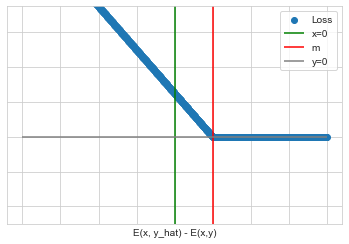
\includegraphics{relu}
The loss as a function of the energy differential $e = E(x_i, \hat{y}_i) - E(x_i, y_i)$ takes on the form of the ReLU function shifted right by $m$ units. We can see that the loss is 0 when the energy differential $e$ is equal to or greater than the margin $m$; when the energy differential $e$ is lower than $m$, then the loss scales linearly with $e$. This is simply because the loss function written as a function of the energy differential is equal to $[m - e]^+$.

\subsection{d}
For one training example $x$, let $Y$ be the matrix of shape $(|T, L|$ where the $(t, l)$th entry contains the probability that the $t$th word is assigned the $l$th part of speech tag. Let $\tilde{y}$ correspond to the vector of shape $|T|$ containing the parts of speech with maximum likelihood for each word given $Y$. Then we could write the inference minimization problem as 

$$ Y = Y - \eta * \nabla_{\tilde{y}} E_\theta (x,\tilde{y})$$

\subsection{e}

\subsubsection{i}
An alternative $\Delta(y, y')$ could be the edit distance between $y$ and $y'$, corresponding to the minimum number of tag changes needed to take $y'$ to $y$. For tags which are especially different, for example tagging a word as a proper noun when the gold standard tag is URL, mismatches or edits taking one to another can be penalized even more. This would more heavily penalize situations where the target tag and the model's next-best tag sequence are extremely different, while allowing the margin between the target tag and a very similar tag to be narrower.

\subsubsection{ii}
Previously, the maximization step only considered the tag sequence with the lowest energy compared to the target tag sequence when choosing which tag sequences to penalize. With Objective 2, the maximization step now considers both the model's inability to create sufficient margin between the target tag sequence and the tag sequence of lowest energy as well as the distance between the tag sequences from the target tag sequence itself. The model must now create a bigger margin between the target tag sequence and tag sequences which are dissimilar to the target in terms of $\Delta$. Tag sequences which are similar to the target tag sequence, on the other hand, are now allowed to have much smaller margins; that is, their energy can be closer to the target tag sequence without incurring a penalty.

\subsubsection{iii}
Objective 2 might allow the energy function to develop a finer-grained concept of similarity between different tag sequences. Previously, there was no real distance function between tags and so even tags which were very similar to the target tag were still forced to be the same distance away as a tag sequence which was completely incorrect. The model could predict the same energy for all tag sequences save the target tag, and achieve the same performance on Objective 1. In Objective 2, the model is forced to assign lower energy to the tag sequences which are closer to the target.

\section{Problem 5}
\subsection{a}
Contrastive, architectural, and regularized methods are three strategies within the EBM framework for assigning low energy regions.

\begin{enumerate}
    \item Contrastive methods manipulate the energy function by pushing down on areas where the energy is desired to be low and pushing up on areas where the energy is desired to be high. These methods generally specify the specific points where the energy based model must have lower and higher energy. Contrastive EBM methods include maximum likelihood, margin-based methods, and the standard cross-entropy loss function.
    \item Architectural methods tend to fix the total amount of low energy space that is available. By assigning regions of low energy, all other regions will naturally have their energy increased. These types of methods include $k$-Means, where the low energy region is near a centroid, as well as Gaussian mixture models.
    \item Regularized methods penalizes having many regions with low energy, and in doing so naturally limits the amount of low energy space. These methods include VAEs and sparse coding models.
\end{enumerate}

\subsection{b}
The free energy $F(y)$ of the sparse coding model is given by

$$F(y) = \min_z ||y -wz||^2 + \lambda|z|_1$$

where $w$ is the decoding matrix, $z$ is the latent code, $y$ is the input which we want to encode, $\lambda$ is a regularizing coefficient on the $l_1$ norm of our latent variable $z$. In English, the free energy $F(y)$ corresponds to the smallest possible energy $E(y,z) = ||y -wz||^2 + \lambda|z|_1$ that can be achieved within the latent encoding space $z$ lies in. The energy function is comprised of two parts: $||y -wz||^2$ is the distance of $y$ to the decoding $wz$ which we want to keep low, and $\lambda|z|_1$ is the size of our latent encoding which we want to keep small.

\subsection{c}
Without any regularizer, the model will just make everything a latent variable $z$ and in doing so will be able to perfectly reconstruct the images at the cost of losing the sparsity that makes the model worth training. The energy will be low everywhere.

\subsection{d}
The regularizer limits the energy function such that it cannot be low everywhere. With the regularizer, an image $i_1$ is considered "high energy" if it is not easily reconstructed using the sparse coding of other images; that is, the image is very unlike the typical image seen in the dataset and it is difficult to use the use a linear combination of the latent variables to reconstruct $i_1$. On the other hand, an image $i_2$ is considered "low energy" if it is very similar to other images which were used as latent variables in the sparse coding model. 

\subsection{e}
$k$-means clustering is an architectural method because it fixes the amount of low energy space that is available by limiting that space to be near the $k$ centroids. The free energy function $F(y)$ is given by 

$$F(y) = \min_z ||y - wz||^2$$

where once again $w$ is a decoding matrix for the latent variables $z$. 

In a $k$-means clustering algorithm, we have a constraint such that there can only be $k$ latent variables. (Contrast with the sparse coding example, where there is no explicit constraint on the number of latent variables because there is a regularization term instead). Thus, our latent variable $z$ is a $k$-dimensional distribution over which centroids $y$ is closest to. The centroids correspond to the columns of the decoding matrix $w$, and the centroids are in the same space as $y$. Let's say $y$ is $m$-dimensional.

Then $y$ is of shape $(m,1)$, the decoding matrix $w$ is of shape $(m,k)$ and holds $k$ centroids of dimension $m$, and the latent variable is of shape $(k,1)$.

\end{document}
